\chapter{Mathematical Representations of Uncertainty}\label{chap:representation_of_uncertainty}

\section{Introduction}
This chapter takes some distance from the stereo vision problem presented previously, and instead describes more formally different representations of uncertainty and the tools that can be used to manipulate them. In this thesis, we consider classical probabilities (\Cref{sec:probabilities}), possibility distributions (\Cref{sec:possibilities}) and p-boxes (\Cref{sec:pboxes}) to model uncertainty. We also consider the case where we have uncertainty on multiple variables simultaneously. In this setting, the dependency between the different sources must be taken into account. We thus present a dependency model called copulas in \Cref{sec:copulas}, and some of its properties. The thorough presentation of those concepts will then be put into relations in \Cref{chap:joining_credal_sets}. 

\section{Notations}
We introduce here a few notations that will be used in this chapter.
\begin{itemize}
    \item \st means ``such that''
    \item We will often present theorems or results with $n$ different variables, spaces, or Cartesian products of $n$ elements. Notations therefore quickly become quite heavy. For that reason, we often use the notation ``$\ldots$'' to imply that we are enumerating all variables. For instance, if we apply a function $f$ to four variables $x_1, x_2, x_3, x_4$, we will write $f(x_1\enum x_4)$.
    \item When working with $n$ variables, the index $i$ will usually be used to refer to the $i$-th variable (or one of its attribute), and will be appended as a subscript when possible, otherwise as a superscript. For instance, if $x\in\mathbb{R}^n$, then $x_i$ will refer to the $i$-th component of $x$. If $m_\times\in\mathbb{R}^n$, then $m_\times^i$ will refer to $i$-th component of $m_\times$.
    \item $\opi\cdot,\cdot\cli$ refers to an interval of integers. For instance $\opi1,~4\cli=\{1,~2,~3,~4\}$.
    \item The power set of a set $\X$ is noted $2^\X$. It corresponds to the set of all sets included in $\X$. In the discrete case, if the cardinal of $\X$ is $n$, then the cardinal of the power set is $2^n$, thus the notation.
\end{itemize}

\section{Different Models to Represent Uncertainty}\label{sec:different_models_of_uncertainty}
Assessing the reliability of an engineering system requires quantifying the uncertainty of the input parameters or of the system itself, using models of uncertainty. Modeling the uncertainty can be done in various ways, depending on the type of uncertainty considered and the available measures or \textit{a priori} regarding the uncertain sources. Most common models are probability distributions, which have been studied extensively. When using those models, we know —or assume— that the information we try to estimate is of stochastic (or random) nature, and that we are able to precisely describe its structure using a probability distribution. However, there are many cases where such assumptions cannot be made: for instance when data is insufficient to determine the correct probability distribution, or when the uncertainty is not random, but epistemic. In those cases, we can use other models, such as:
\begin{itemize}
    \item fuzzy sets \cite{zadeh_fuzzy_1999} when trying to estimate the degree of truth of a statement such as ``This person is tall''
    \item intervals \cite{jaulin_applied_2001}, where no preferences are given inside a specific range of possible values
    \item \acrfull{ip} which tries to extend the concept of probabilities in order to model epistemic uncertainty \cite{augustin_introduction_2014}
\end{itemize}
This list is not exhaustive. Additionally, those different models can sometimes be equivalent. Choosing to use one or another depends on the nature of the problem and of the available data. In this chapter, we will mainly consider probability distributions (\Cref{sec:probabilities}) and \acrshort{ip} (\Cref{sec:imprecise_probabilities}). Two specific cases of \acrshort{ip} will be detailed, namely possibility distributions in \Cref{sec:possibilities} and p-boxes in \Cref{sec:pboxes}.

\begin{remark}
    Distinguishing between stochastic and epistemic uncertainty is a model accepted by many to distinguish between different situations of uncertainty. One could argue that stochastic uncertainty is, to some extent, equivalent to epistemic uncertainty. Indeed, if we had enough knowledge on initial conditions of a die throw for instance (force and torque applied on the dice, its exact shape and mass distribution \etc), as well as the exact physics model, one could predict with certainty on which side it would land. There would therefore be no aleatoric process at stake here. The question whether or not we should make the distinction between aleatoric and epistemic uncertainty is of interest regarding theoretical aspects of the nature of uncertainty. For real-life applications, however, differentiating between the two seems reasonable, as we cannot know every parameter and the exact model involved for every quantity of interest. 
\end{remark}

At the end of the day, choosing one model over another is not always straightforward. It requires being aware of the type of uncertainty faced, of the strengths and limitations of each model, of the tools available to manipulate the models \etc When it comes to less common models cited above, it fundamentally requires being aware of the existence of such models, which is not always the case for non-specialists. During this thesis, we tried to promote less common models, especially possibility distributions. We did so by presenting real life cases where they could be used while improving uncertainty modeling in the field of stereophotogrammetry (see \Cref{chap:propagating,chap:epistemic_uncertainty}).

\subsection{Probabilities}\label{sec:probabilities}
Probability measures are a classical framework to represent uncertainty. There are multiple ways of interpreting them, mainly with a \textit{frequentist} approach, or a \textit{Bayesian} approach. From a frequentist point of view, probabilities are well-fitted to represent stochastic uncertainty, \ie uncertainty regarding events that can get a different result each time we run an experiment or acquire a measure (typically, noise on a sensor). From a \textit{Bayesian} point of view, probabilities represent a state of knowledge or degree of belief, and can be updated with additional information \cite{irvine_philosophies_2009}. This leads to the notion of prior and posterior probability that will not be considered in this thesis.

We remind here basic definitions regarding probability distributions.

\begin{definition}[Probability Space]\label{def:probability_space}
    We call a probability space $(\X,~\mathcal{A},~P)$ a tuple where:
    \begin{itemize}
        \item $\X$ is the set of possible outcomes (for instance, head or tails for a toss coin)
        \item $\mathcal{A}$ is the set of all subsets of $\X$ for which a probability can be measured (for instance $\{\emptyset, \{\text{heads}\}, \{\text{tails}\}, \{\text{heads, tails}\}\}$)
        \item $P$ is the probability measure assigning a probability to each of the sets of $\mathcal{A}$. For instance, for a fair coin, $P(\emptyset)=0$, $P(\{\text{heads}\})=P(\{\text{tails}\})=0.5$ and $P(\X)=1$.
    \end{itemize}
    Note that $\mathcal{A}$ must be a $\sigma$-algebra, meaning that it is closed under complement, countable unions and countable intersections. $P$ is a probability measure if it verifies all the Kolmogorov axioms:
    \begin{itemize}
        \item $\forall A\in\mathcal{A},~P(A)\in[0,1]$
        \item $P(\X) = 1$
        \item for any countable disjoint family of sets $A_i\in\mathcal{A}$, $P(\cup_i A_i)=\sum_i~P(A_i)$
    \end{itemize}
\end{definition}

\begin{definition}[Random Variable]
    A random variable $X$ is a measurable function from $\X$ to a measurable space (which is $\mathbb{R}$ or a subset of $\mathbb{R}$). We can then measure the probability that $X$ takes its values in a measurable set $E\subseteq\mathbb{R}$:
    \begin{align*}
        P(E) = P(\{x\in\X~|~X(x)\in E\})
    \end{align*}
\end{definition}

Using a random variable allows considering the probability measure on different spaces. We then call $P$ the probability distribution of the considered random variable $X$.

Other useful concepts regarding probability distributions are \acrfull{pdf} and \acrfull{cdf}:
\begin{definition}[Cumulative Distribution Function]\label{def:cdf}
    A \acrfull{cdf} $F_X$ of a random variable $X$ with real values is the probability that $X$ will be less or equal to a number $x$. Formally, we define $F_X:\X\rightarrow[0,1]$:
    \begin{equation*}
        \forall x\in\X,~F_X(x)=P(X\leqslant x)
    \end{equation*}
\end{definition}

\begin{definition}[Density Function]\label{def:density}
    A random variable $X$ is said to possess a \acrfull{pdf} if there exists a positive integrable function $f$ over $\mathbb{R}$ \st $\forall (x_1, x_2)\in\mathbb{R}^2$:
    \begin{equation*}
        P(x_1\leqslant X \leqslant x_2) = \int_{x_1}^{x_2}f(x)dx
    \end{equation*}
    In the continuous case, the \acrshort{pdf} $f$ is also the derivative of the \acrshort{cdf} of $X$. In the discrete case, the \acrshort{pdf} is also called \textit{probability mass function}, and is defined as:
    \begin{equation*}
        f(x_1) = P(X = x_1)
    \end{equation*}
\end{definition}

In the rest of the chapter, we consider random variables $X$ on discrete spaces $\X$. If $\X=\{x_1,~\ldots,~x_n\}$, we call $\{x_i\}$ an atom of $\X$, and the probability distribution $P$ of $X$ on $\X$ is completely determined by its \acrshort{pdf}, which is the value of $P$ on atoms. For simplicity of notation, we will not always use braces around atoms when computing their probability. So we will sometimes write $P(x_1)$ instead of $P(X=\{x_1\})$.

As stated previously, probability measures are fitted to represent stochastic uncertainty. The following example illustrates why probability measures are not adapted to represent epistemic uncertainty:

\begin{example}\label{ex:proba_limitations}
    Let consider a card facing down, with a number written on its hidden side. The person who wrote the number tells you that they chose to write either $1$, $2$ or $3$ on it. We should note that because they chose to write a number, the uncertainty on its value is not random. They then ask you to evaluate your chances of guessing the correct number and its parity, \ie if it is odd or even. We first consider the random variable $X$ taking values in $\{1,~2,~3\}$. Because you have no further information and thus no preferences on the values of $X$, a common (yet arguably inadequate) decision is to associate the uniform distribution $P$ to $X$:
    \begin{equation*}
        P(X=1)=P(X=2)=P(X=3)=\frac{1}{3}
    \end{equation*}
    Concerning the parity of the number, we may consider the random variable $Y$ defined such that $Y=0$ if ``$X=1$ or $X=3$'' and $Y=1$ if ``$X=2$''. Because we have no information on the number written on the card, we also do not have any preferences on the values of $Y$. Following the same reasoning as before, one might be tempted to associate a uniform distribution to it. However, deducing the \acrshort{pdf} of $Y$ from that of $X$ yields:
    \begin{equation*}
        P(Y=0)=P(X=1)+P(X=3)=\frac{2}{3},\qquad P(Y=1)=P(X=2) = \frac{1}{3}
    \end{equation*}
    which is clearly not the \acrshort{pdf} of a uniform distribution. By assuming we have no preferences on the values of a variable, we actually deduced preferences on the values of another variable. 
    
    This example shows that one should use a uniform distribution only when they are certain that all values are equiprobable. This is due to the fact that uniform distributions are well suited for representing statements like ``all values have the same likelihood'' but not for statements like ``I have no information over the values, and thus no preference''. Indeed, a probability distribution actually contains a lot of information about a (random) variable, which is not suited to represent epistemic uncertainty.
    
    \begin{remark}
        From a Bayesian point of view, a probability can also represent a degree of belief, allowing them to represent epistemic uncertainty and not only stochastic uncertainty, in theory. However, it does not solve the expressiveness problem raised by this example. Bayesians are still reasoning with probabilities, which make no difference between ``I have no preference between these events'' and ``these events are equiprobable''. Even though they can update their prior with additional information, this would not fix the problem presented here. In the absence of additional information, basing a decision on the prior would lead to debatable conclusions.
    \end{remark}
\end{example}

\subsection{Imprecise Probabilities}\label{sec:imprecise_probabilities}
As highlighted in \Cref{ex:proba_limitations}, uncertainty cannot always be correctly modeled by probabilities, especially in a context where data is sparse. To overcome this problem, a generalization of probabilities has been introduced, called \acrfull{ip}, which provides a general framework for working with both aleatoric and epistemic uncertainty. It uses the concept of lower and upper probabilities, which are quite generic and flexible, and can be derived in more specific models. Here is a brief scope of the relevant tools it encompasses: the special case of \textit{belief functions}, themselves containing specific sub-categories such as possibility distributions (\Cref{sec:possibilities}) and probability boxes (\Cref{sec:pboxes}). It also contains probabilities presented in \Cref{sec:probabilities}, which we will call \textit{precise} probabilities in contrast to \textit{imprecise} probabilities. \Cref{fig:diagram_IP} is a non-exhaustive overview of relationships and specificities of each imprecise model.

\begin{remark}
    On a more generic level, \acrshort{ip} can be described by sets of acceptable gambles and by lower and upper expectations \cite{walley_statistical_1991,augustin_introduction_2014}. Although very interesting, we did not use them in our applications and thus do not consider them in this thesis.
\end{remark}

\begin{figure}[ht]
    {\centering
    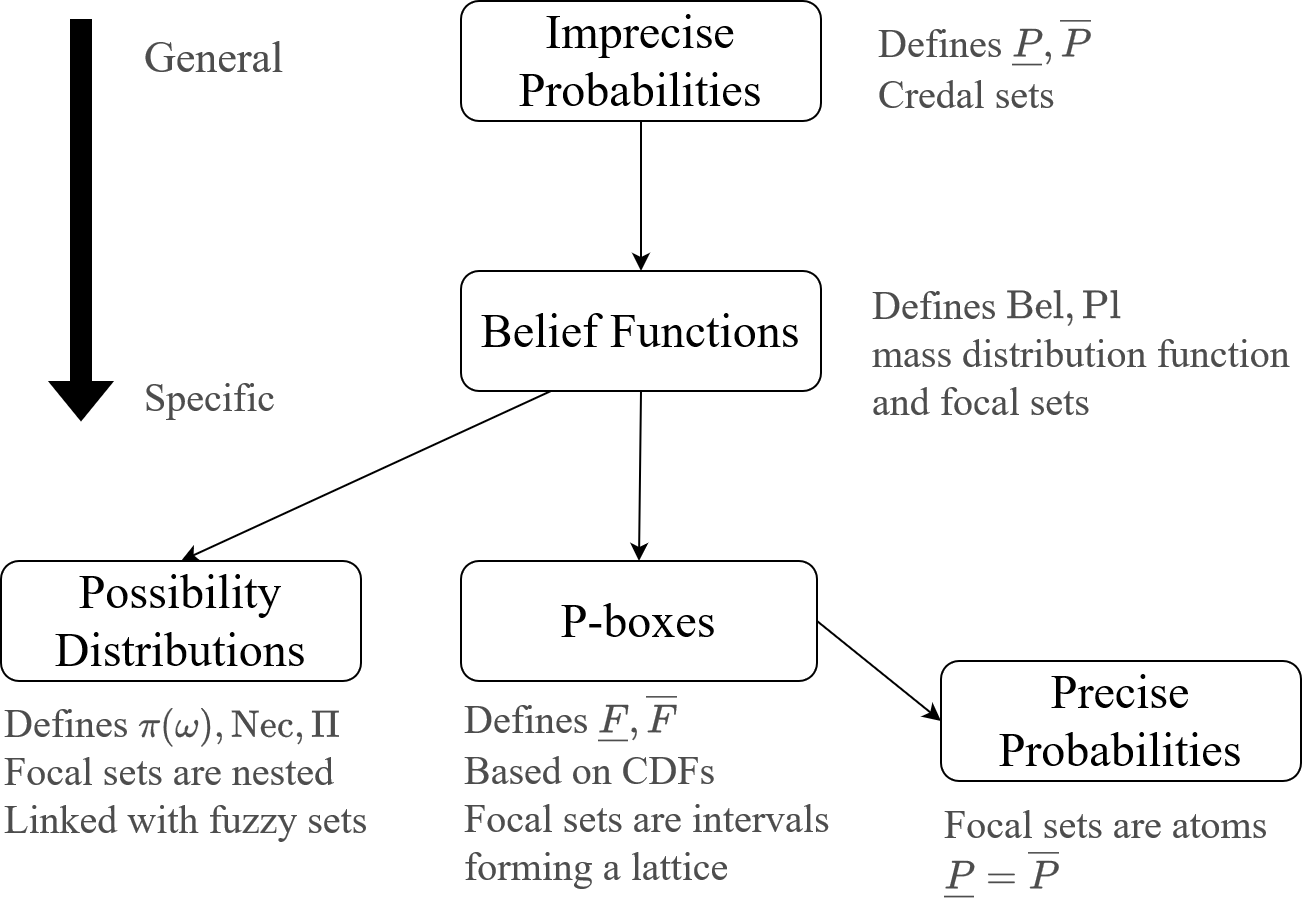
\includegraphics[width=0.8\linewidth]{Images/Chap_2/Diagramme_IP_Bel.png}
    \caption{Diagram representing the relationship between different \acrshort{ip} models presented throughout \Cref{sec:different_models_of_uncertainty}.}
    \label{fig:diagram_IP}}
\end{figure}

As stated previously, a core concept of \acrshort{ip} is the concept of lower and upper probabilities. Similarly to precise probabilities, a lower probability $\low$ and an upper probability $\overline{P}$ are mappings from a $\sigma$-algebra $\mathcal{A}$ to $[0, 1]$. However, while a probability $P$ gives a single measure of uncertainty for every event, lower and upper probabilities provide two bounds for every event, allowing them to express more complex uncertainty structures.

\begin{remark}
    Formally, a lower probability $\low$ needs to be \textit{super-additive}, \ie to satisfy:
    \begin{equation}
        \forall A,B\in\mathcal{A}, \text{ if } A\cap B\neq\emptyset, ~\low(A\cup B)\geqslant \low(A)+\low(B) \label{eq:super_additivity}
    \end{equation}
    Conversely, an upper probability is sub-additive, meaning that it verifies the same property as \Cref{eq:super_additivity} but with the inequality reversed.
    
    Those properties are less constraining than their equivalent for precise probabilities in \Cref{def:probability_space}, so lower and upper probabilities are generally \textit{not} precise probabilities. The only case where they are precise probabilities is when $\low=\overline{P}$, because $\low$ is then additive as it is both super and sub-additive. In this case, \acrshort{ip} are actually a single precise probability. This illustrates the fact that precise probabilities are special cases of \acrshort{ip}. 
\end{remark}

Precise probabilities define a measure of uncertainty towards a random variable $X$ taking numerical values. \acrshort{ip} however, can model the uncertainty towards a random variable taking set values instead of numerical one. We then say that $X$ is a \textit{random set} instead of a random variable. That being said, \acrshort{ip} can also represent the uncertainty of random variables for which we assume a precise probability exists, but we are not able to determine it precisely. Indeed, lower and upper probabilities form the bounds of a family of precise probabilities called \textit{credal set}.
\begin{definition}[Credal set]\label{def:credal_set}
    Given a lower probability $\low$ and an upper probability $\overline{P}$, a credal set $\M$ is the set of all probabilities $P$ that are greater that $\low$ and lower that $\overline{P}$:
    \begin{equation}
        \M(\low, \overline{P}) = \{P~|~\forall A\in\mathcal{A},~\low(A)~\leqslant~P(A)~\leqslant\overline{P}(A)\}
    \end{equation}
\end{definition}
We refer to $\M(\low, \overline{P})$ as $\M$ when no confusion is possible. Credal sets allow considering multiple probabilities at once, which improves on the limited expressiveness of a single probability measure. The gap between the two bounds of a credal set reflects how imprecise is the model, in terms of epistemic uncertainty.

Conversely, we can define lower and upper bounds from a set of probabilities $\M$ as:
\begin{align*}
    \forall A\in\mathcal{A},~\low(A) =& \inf_{P\in\M}P(A)\\
    \forall A\in\mathcal{A},~\overline{P}(A) =& \sup_{P\in\M}P(A)
\end{align*}
Note that $\M$, contrary to $\M(\low, \overline{P})$, is not necessarily defined by $\low, \overline{P}$. Therefore, even though $\M$ and $\M(\low,\overline{P})$ have the same bounds on events, they are not necessarily equal and only $\M\subseteq\M(\low, \overline{P})$ holds. 

Although it is not required, we usually assume that credal sets verify additional properties expressed as follows:
\begin{definition}[Coherence and Avoiding sure loss]\label{def:coherence_sure_loss}
    A credal set $\M$ is said to avoid sure loss if it contains at least one probability measure, \ie if
    \begin{equation}
        \M \neq \emptyset\label{eq:avoid_sure_loss}
    \end{equation}
    
    In this thesis, we consider that a credal set $\M$ induces \textit{coherent} lower and upper probabilities if its lower and upper bounds on all events are attained by a probability measure, \ie if:
    \begin{equation}
        \forall A\in\mathcal{A}, \exists P, P'\in\M~\st~\low(A)=P(A) \text{ and } \overline{P}(A)=P'(A) 
    \end{equation}
\end{definition}
The bounds $\low, \overline{P}$ of a coherent credal set verify the following property:
\begin{equation}
    \forall A\in\mathcal{A}, ~\low(A) = 1 - \overline{P}(A^c)\label{eq:lower_proba_complement}
\end{equation}
which is a generalization of the classical property for computing the complement of an event with precise probabilities. This allows us to only specify the lower bound $\low$ of a credal set to completely describe it, as its upper bound is determined by $\low$ through complementation. Defining a credal set requires specifying much more constraints on the probability space than in the case of probability distributions. Indeed, a lower probability must be defined on every possible event, while a precise probability can be defined by its \acrshort{pdf} on possible values only (instead of possible events). In the case of a discrete space with $n$ elements, a probability is completely determined by its values on the $n$ atoms, while a lower bound is completely determined by its values on the $2^n$ considered events.


\begin{remark}
    Sampling from a credal set is not straightforward. Multiple methods exist, the most intuitive consisting in sampling distributions from the credal set extreme points.
\end{remark}

\begin{remark}
    With the way we defined a credal set $\M$, it is closed and convex. This is a common way of constructing credal sets, but is not the only way. We could for instance impose that all probabilities in $\M$ belong to a family of Gaussian probabilities, which would prevent $\M$ from being convex.
\end{remark}

When constructing credal sets, it is common to possess a non-convex set of probabilities $S$. In that case, we can define the convex hull of a set of probabilities $S$:
\begin{definition}[Convex Hull]\label{def:convex_hull}
    The convex hull ($CH$) of a set of probabilities $S$ is the smallest (convex) credal set containing $S$.
\end{definition}

\begin{remark}
    The convex hull is computationally heavy to evaluate. Determining the infimum and supremum of a set of probability is not trivial, as it might be required to iterate through every element of $S$. It is however very useful, especially in the case where we do not know the set bounds on every event. In that case, computing the convex hull also allows us to determine the bounds on those events.
\end{remark}

\begin{example}
    Let us consider the scenario presented in \Cref{ex:proba_limitations} and model the uncertainty with a credal set instead of a single probability distribution. Because we have no information on the value written on the card except that it is in $\{1,2,3\}$, we characterize the uncertainty by lower and upper probability $\low$, $\overline{P}$ defined as follows:
    \begin{align*}
        &\low(X=1) = \low(X=2)= \low(X=3) = 0\\
        &\overline{P}(X=1) = \overline{P}(X=2)= \overline{P}(X=3) = 1\\
        &\low(X\in\{1,2,3\}) = \overline{P}(X\in\{1,2,3\}) = 1
    \end{align*}
    We can use \Cref{eq:lower_proba_complement} for computing the bounds of remaining events.
    
    Here, the credal set is the largest credal set possible, as its bounds are always $0$ and $1$ for events that are not $\emptyset$ or $\{1,2,3\}$. We say that it is the vacuous credal set, as it does not encode any information. It however solves the problem of a contradicting probability when evaluating the value of the card and its parity presented in \Cref{ex:proba_limitations}
\end{example}

\subsection{Belief Functions}\label{sec:belief_functions}
A special case of \acrshort{ip} are belief functions, which we will detail in this section. First, we will introduce a key concept that goes along belief functions: mass distribution functions. We will then derive belief functions from it.

\begin{definition}[Mass distribution function]\label{def:mass_distribution_function}
    Let $\X$ be a set of possible outcomes, and $2^\X$ its power set. A mass distribution function (or basic probability assignment \cite{shafer_mathematical_1976}) is a function $m:2^\X\rightarrow[0,1]$ \st:
    \begin{align}
        m(\emptyset) =& 0\label{eq:mass_emptyset}\\
        \sum_{a\subseteq\X}m(a) =& 1\label{eq:mass_whole_set}
    \end{align}
\end{definition}

There are multiple ways of interpreting $m(a)$, presented as follows:
\begin{itemize}
    \item If we consider a random set $X$, then $m(a)$ encodes the probability mass that $X$ takes $a$ as its set value.
    \item If $X$ is a random variable, then $m(a)$ encodes the available evidence that the numerical value of $X$ is \textit{exactly} in $a$, without any preferences for the values within $a$. This means there could also be other evidence that $X$ is in $a'\subset a$, encoded with $m(a')$, and which could be either more or less than $m(a)$ depending on the amount of evidence available. \Cref{ex:bicycle_pressure} illustrates this with a toy scenario. 
    \item $m(a)$ can also be linked to precise probability masses defined in \Cref{def:density}. If we assume there exists an unknown underlying probability measure $P$ for $X$, $m(a)$ measures the probability mass that is assigned to $a$, but that can move freely to every point of $a$ without any preference. In other words, with more information, we could distribute $m(a)$ to every element of $a$, and doing this for all $a$ would lead to a precise probability mass distribution.
\end{itemize}

\begin{remark}
    \Cref{eq:mass_emptyset} translates the fact that there is no evidence that the uncertain variable belongs to the empty set, \ie that it is not defined. Relaxing this constraint allows accepting a certain amount of contradiction in our model.
    \Cref{eq:mass_whole_set} is a convention, which states that the total amount of evidence equals $1$. It is similar to probabilities, which cannot be more than $1$. 
\end{remark}

\begin{definition}[Focal set]\label{def:focal_set}
    Let $\X$ be a set of possible outcomes, $2^\X$ its power set, and $m:2^\X\rightarrow[0,1]$ a mass distribution function. A set $a\subseteq\X$ is called a focal set of $m$ if and only if:
    \begin{align}
        m(a)>0\label{eq:focal_set}
    \end{align}
\end{definition}
Focal sets thus represent sets of the set of possible outcomes for which we have evidence. The set of all focal sets is sometimes referred to as the \textit{core} of $m$.

\begin{definition}[Belief function, Plausibility function]\label{def:belief_plausibility}
    Let $\X$ be the set of possible outcomes, $2^\X$ its power set, and $m:2^\X\rightarrow[0,1]$ a mass distribution function.
    
    We define the belief function associated with $m$ as the function $\Bel:2^\X\rightarrow[0,1]$ who associates to all events $A$ in $2^\X$:
    \begin{align*}
        \Bel(A)=\sum_{a\subseteq A} m(a)
    \end{align*}
    
    We define the plausibility function associated with $m$ as the function $\Pl :2^\X\rightarrow[0,1]$ who associates to all events $A$ in $2^\X$:
    \begin{align*}
        \Pl(A)=\sum_{\substack{a\\a\cap A\neq\emptyset}} m(a)
    \end{align*}
    $\Bel$ and $\Pl$ are special cases of lower and upper probabilities, and thus induce a credal set $\M(\Bel, \Pl)$ defined as:
    \begin{align*}
        \M(\Bel, \Pl) =\{P~|~\forall A\subseteq\X, \Bel(A) \leq P(A) \leq \Pl(A) \}
    \end{align*}
\end{definition}
We can interpret $\Bel(A)$ as the amount of evidence that fully support $A$, and $\Pl(A)$ as the amount of evidence that is consistent (or does not contradict) with $A$.

$\Bel$ and $\Pl$ are special cases of lower and upper probabilities, and verify \eqref{eq:lower_proba_complement} as for all events $A$ it holds:
\begin{align*}
    \Bel(A)&=\sum_{a\subseteq A} m(a)\\
    &= \sum_{a\in \X} m(a) - \sum_{a\not\subseteq A} m(a)\\
    &= 1 - \sum_{\substack{a\\a\cap A^c\neq\emptyset}} m(a)\\
    &=1-\Pl(A^c)
\end{align*}
Because $\Pl$ is completely determined by $\Bel$ through complementation, we will refer to $\M(\Bel,\Pl)$ simply as $\M(\Bel)$.

Belief functions possess interesting properties, making the credal set they induce both coherent and avoiding sure loss, motivating their extensive usage.

\begin{example}[Defining mass and belief functions]\label{ex:bicycle_pressure}
    Let us imagine an experiment where you try to estimate the pressure of the tires of your bike, but your bicycle pump only have graduation every $1$ bar. You are able to do three measurements:
    \begin{itemize}
        \item The first measure, the needle seems to be between $4$ and $5$ bar.
        \item The second measure, the needle seems to be between $4.5$ and $6$ bar.
        \item The third measure, the needle seems to be between $4.5$ and $5.5$ bar.
    \end{itemize}
    Let us say that you trust your last measurement the most, because you got used to the movement of the needle. It is now possible to model the uncertainty of your tire pressure using available evidence, encoded in $m$:\newline
    \begin{minipage}{0.3\textwidth}
        \begin{align*}
            m([4,~5]) ~=~ 0.3
        \end{align*}
    \end{minipage}\hfill
    \begin{minipage}{0.3\textwidth}
        \begin{align*}
            m([4.5,~6]) ~=~ 0.3
        \end{align*}
    \end{minipage}\hfill
    \begin{minipage}{0.3\textwidth}
        \begin{align*}
             m([4.5,5.5]) ~=~ 0.4
        \end{align*}
    \end{minipage}\bigskip\newline
    Based on this, we are now able to express our degree of belief and of plausibility for all events. For instance:
    \begin{itemize}
        \item Our degree of belief that the pressure lies in $[4, 5]$ is $\Bel([4, 5])=0.3$, that it lies in $[4, 5.5]$ is $\Bel([4, 5.5])=0.7$ and that it lies in $[4, 6]$ is $\Bel([4, 6])=1$
        \item The degree of plausibility that the pressure equals $5$ is $\Pl (5)=1$ (totally plausible), that it equals $5.5$ is $\Pl (5.5)=0.7$ and that it equals $4$ is $\Pl (4)=0.3$.
    \end{itemize}
\end{example}

\subsection{Possibility Distributions}\label{sec:possibilities}
Other convenient models of uncertainty are possibility distributions, which are a specific case of imprecise probabilities, as presented in \Cref{fig:diagram_IP}. We will see that they induce a particular type of belief functions, and will be used in our applications.

\begin{definition}[Possibility distribution]\label{def:possibility}
    Let $\X$ be the set of possible outcomes. A possibility distribution is a function $\pi: \X \rightarrow [0,1]$ satisfying:
    \begin{equation}
    	\exists x \in \X, \pi(x) = 1 \label{eq:possibility}
    \end{equation}
    The value $\pi(x)$ represents the degree of possibility of $x$, with $\pi(x) = 1$ indicating full possibility, and $\pi(x) = 0$ indicating impossibility.
\end{definition}

Another notion closely related to possibility distributions is that of \(\alpha\)-cuts:
\begin{definition}[\(\alpha\)-cut]\label{def:alpha_cut}
    Let $\pi: \X \rightarrow [0,1]$ be a possibility distribution. Given any \(\alpha\in[0,1]\), we define the \(\alpha\)-cut of \(\pi\) as:
    \begin{align}
        \alpha_\pi=\{x~|~\pi(x)\geqslant\alpha\} \label{eq:alpha_cut}   
    \end{align}
    An \(\alpha\)-cut is thus the set of all elements of $\X$ whose possibility level is more than $\alpha$.
\end{definition}

\begin{definition}[Necessity and Possibility measures]\label{def:possibility_credal_set}
    It has been proven in \cite{dubois_when_1992} that a possibility distribution defines a specific type of plausibility functions called \textit{possibility} function and noted \(\Pi\). It also defines a specific belief function by duality called \textit{necessity} function and noted \(\Nec\), as well as a credal set $\M(\pi)$. They are defined as:
    \begin{align}
        \Pi(A) &= \sup_{x\in A}\pi(x)\\
        \Nec(A)& =1-\sup_{x\in A^c}\pi(x)\label{eq:bel_pl}\\
        \M(\pi)& =\{P~|~\forall A,~P(A)\leqslant \sup_{x\in A}\pi(x)\}\\
        &=\{P~|~\forall A,~P(A)\leqslant \Pi(A)\} \label{eq:credal_set_possibility}\\
        &= \{P~|~\forall A,~P(A)\geqslant \Nec(A)\}
\end{align}
\end{definition}

\begin{example}[Defining a possibility distribution]\label{ex:bicycle_pressure_possibility}
    Let us imagine the same setting as \Cref{ex:bicycle_pressure}, where we try to estimate the pressure of the tires of our bike, but our bicycle pump only has graduations every $1$ bar. We are able to do the following measurements:
    \begin{itemize}
        \item During the first measurement, the needle seems to be around $4$ bar.
        \item During the second measurement, the needle seems to be around $5$ bar.
        \item During the third measurement, the needle seems to be around $4.5$ bar.
    \end{itemize}
    Let us say that we trust our measurement with a precision of $\pm0.5$ bars. For simplicity, we also only consider pressure values that are integers or half integers. Taking into considerations all the measurements, we can define a possibility distribution $\pi$ as:
    \begin{itemize}
        \item The value of $4.5$ being the most possible, $\pi(4.5)=1$.
        \item Values between $4$ and $5$ bar being highly possible, we can for instance fix $\pi(4)=\pi(5)=0.8$
        \item Values $3.5$ and $5.5$ are unlikely but not impossible, we can say that $\pi(3.5)=\pi(5.5)=0.3$
        \item Other values are impossible, thus they have a possibility of $0$.
    \end{itemize}
    The possibility distribution $\pi$ is represented in \Cref{fig:possibility_distribution}. 
    Based on this, we are now able to express the degree of necessity and possibility for all events. For instance:
    \begin{itemize}
        \item The degree of necessity that the pressure lies between $4$ and $5$ bar is $\Nec([4, 5])=1-\sup_{\rho\not\in[4,5]}\pi(\rho)=0.7$
        \item The degree of necessity that the pressure lies between $3.5$ and $5.5$ bar is: 
        \begin{align*}
            \Nec([3.5,~ 5.5]) = 1-\sup_{\rho\not\in[3.5,5.5]}\pi(\rho) = 1
        \end{align*}
        meaning that the pressure is necessarily in this range.
        \item The degree of possibility that the pressure is either $3.5$ or  $5$ is $\Pi (\{3.5,~5\})=\sup_{\rho\in\{3.5,~5\}}\pi(\rho)=0.9$ (mostly possible).
        \item \etc for every possible event.
    \end{itemize}
\end{example}

\begin{figure}[!ht]
    \centering
    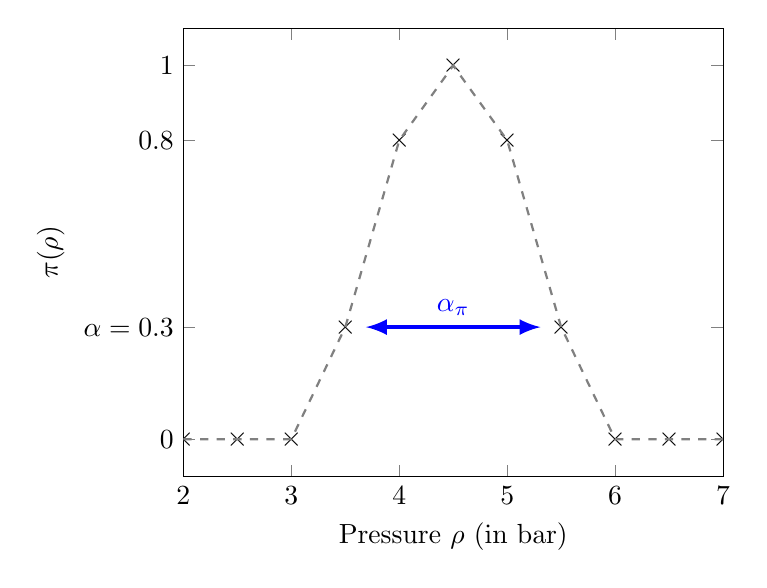
\begin{tikzpicture}[scale=1]
        \begin{axis}[%
          xlabel=Pressure $\rho$ (in bar),
          ylabel=$\pi(\rho)$,
          xmin=2, xmax=7,
          ymin=-0.1, ymax=1.1,
          ytick={0, 0.3, 0.8, 1},
          yticklabels={$0$, $\alpha=0.3$, 0.8, $1$},
          ],
          \node (a) at (2, 0) {$\times$};
          \node (b) at (2.5, 0) {$\times$};
          \node (c) at (3, 0) {$\times$};
          \node (d) at (3.5, 0.3) {$\times$};
          \node (e) at (4, 0.8) {$\times$};
          \node (f) at (4.5, 1) {$\times$};
          \node (g) at (5, 0.8) {$\times$};
          \node (h) at (5.5, 0.3) {$\times$};
          \node (i) at (6, 0) {$\times$};
          \node (j) at (6.5, 0) {$\times$};
          \node (k) at (7, 0) {$\times$};
          
          \draw [thick, dashed, gray] (a.center) -- (b.center) -- (c.center) -- (d.center) -- (e.center) -- (f.center) -- (g.center) -- (h.center) -- (i.center) -- (j.center) -- (k.center) ;
          \draw [<->, >=latex, ultra thick, blue] (d.east) -- (h.west) node [pos=0.5, above] {$\alpha_\pi$};
        \end{axis}
    \end{tikzpicture}
    \caption{Possibility distribution of \Cref{ex:bicycle_pressure_possibility} and one of its $\alpha$-cut in blue}
    \label{fig:possibility_distribution}
\end{figure}

\begin{remark}
    If you are familiar with fuzzy sets, you may have noticed that possibility distributions are similar to membership functions of a fuzzy set. Links between fuzzy sets and possibility measures have been explored in \cite{zadeh_fuzzy_1999}.
\end{remark}

Focal sets of necessity functions can be determined directly from the possibility distribution by looking at their \( \alpha \)-cuts. It has been proven that the core $\mathcal{C}$ (the set containing all focal sets) of a necessity function is (\cite{couso_necessity_2001}):
\begin{align*}
    \mathcal{C} =& \{\alpha_\pi~|~\alpha\in[0,1]\}\\
    =& \{ ~\{x\in\X~|~\pi(x)\geqslant\alpha\}~|~\alpha\in[0,1]~\}
\end{align*}
With the way focal sets are defined, they form a nested family of sets with regard to inclusion. Indeed, if an element of \(\X\) belongs to an \(\alpha\)-cut, then its possibility is greater than \(\alpha\) and therefore belongs to any other \(\alpha'\)-cut with a lower \(\alpha'\). For simplicity, we will assume that the focal sets \(a_1\enum a_n\) are already numbered using the inclusion order, \ie \( a_1\subset\ldots\subset a_n\). In this case, we will refer to the inclusion order as the ``natural'' order for possibility distributions.

\begin{remark}
    The fact that focal sets form a nested family of sets in the case of possibility distributions also implies that if $\X$ is finite and contains $n$ elements, then there can be \textit{at most} $n$ focal sets. For comparison, belief functions can have a maximum of $2^n-1$ focal sets (as the empty set cannot be a focal set). This means that necessity functions have fewer degrees of freedom than (some) belief functions, and thus can express fewer uncertainty structures. This drawback comes with the advantage of being more straightforward to construct, as we only need to specify the mass of $n$ focal sets (or the possibility of the $n$ elements of $\X$) instead of $2^n-1$. Indeed, when we think of a random variable like the outcome of a die, it can seem more natural for someone to specify degrees of possibility for each side separately than it is to specify degrees of plausibility for different sets of outcomes. 
    
    As such, possibility distribution have been used to model experts' opinion in domain such as water contamination \cite{bardossy_l-_1995}, soil contamination and radioactive risk assessment \cite{baudrit_comparing_2005,baudrit_representation_2005,baudrit_joint_2007} or weather forecasting \cite{le_carrer_beyond_2021}. Following the same philosophy, we will use possibility distributions in \Cref{chap:epistemic_uncertainty} to model the uncertainty of a measure of similarity between two image patches.
\end{remark}

Specifying a probability distribution often comes down to specifying the probability mass function over all atoms of the set of possible outcomes. In a way, possibility distributions are constructed the same way, as we specify the possibility (or the upper bounds) of every atom. One important difference is that the condition ``the sum of all masses must be equal to $1$'' is relaxed into a less constraining condition ``the possibility distribution must be equal to $1$ at least once''. In that respect, it is easier to construct a well-defined possibility distribution than it is to construct a well-defined probability distribution. However, the comparison stops there, as the two models does not represent the same type of uncertainty.

\begin{remark}
    Any probability distribution $P$ is a belief function $\Bel$, for which focal sets are only composed of singletons (atoms) and the mass distribution function of $\Bel$ equals the probability mass function of $P$ on atoms. However, a possibility distribution cannot model a probability distribution. Indeed, this would impose that its necessity $\Nec$ and plausibility $\Pi$ functions verify:
    \begin{align*}
        \forall A, &~\Nec(A) = \Pi(A)\\
        \Leftrightarrow&~1-\sup_{x\in A^c}\pi(x) = \sup_{x\in A}\pi(x)\\
        \Leftrightarrow&~ \sup_{x\in A}\pi(x) + \sup_{x\in A^c}\pi(x) = 1
    \end{align*}
    Consider this equation for any $x'$ verifying $\pi(x')=1$. This leads to the conclusion that any $x\neq x'$ has a possibility of $0$, implying that it is impossible for a random set or random variable to take any other value than $x'$, rendering it not-random. 
\end{remark}

\subsection{P-boxes}\label{sec:pboxes}
Another special type of belief function that is commonly used is that of \textit{probability boxes}, more commonly called p-boxes. Formally, a p-box is a pair of precise cumulative distribution functions $[\underline{F}, ~\overline{F}]$ defining lower and upper bounds on all cumulative events:

\begin{definition}[P-box]\label{def:p-box}
    Let $\X$ be the set of possible outcomes. A p-box is a pair of \acrshort{cdf}s $[\underline{F}, ~\overline{F}]$ from $\X$ to $[0, ~1]$ such that:
    \begin{equation}
    	\forall x \in \X,~\underline{F}(x) \leqslant \overline{F}(x) \label{eq:p-box}
    \end{equation}
    If $\X$ is not a subset of $\mathbb{R}$, then there must exist a total order on $\X$ to define a generalized p-box \cite{destercke_unifying_2008}. 
\end{definition}

\begin{remark}
    A probability distribution can be both determined by specifying its values on every atom or by specifying its values on cumulative events. We saw in \Cref{sec:possibilities} that possibility distributions are defined by bounds on atoms. Because p-boxes are defined by bounds on cumulative events, we could say that a p-box is the ``imprecise way'' of defining a probability using cumulative events, and a possibility distribution is the ``imprecise way'' of defining a probability using atoms.
\end{remark}

The credal set $\M$ induced by a p-box $[\underline{F}, ~\overline{F}]$ is:
\begin{align}
    \M([\underline{F}, ~\overline{F}]) = \{~ F ~|~ \forall x\in\X, ~\underline{F}(x)\leqslant F(x)\leqslant \overline{F}(x) ~\}
\end{align}

\begin{definition}[Focal sets of p-boxes]
    P-boxes are special cases of belief functions. It has been proven in \cite{destercke_unifying_2008} that focal sets of p-boxes have a specific form. Although focal sets shapes are reminiscent of possibilities' $\alpha$-cuts (see \Cref{fig:p-box}), they are a bit more complex to express formally. If $\X=\{x_1\enum x_n\}$ with $x_1\leqslant\ldots\leqslant x_n$, then focal sets $\alpha_{[\underline{F}, ~\overline{F}]}$ of $[\underline{F}, ~\overline{F}]$ are given for every $\alpha\in[0,~1]$ by the following expression:
    \begin{align}
        \alpha_{[\underline{F}, ~\overline{F}]}= \opi \overline{F}^{-1}(\alpha),~\underline{F}^{-1}(\alpha)\cli\label{eq:pbox_focal_set}
    \end{align}
    where $\opi\cdot,~\cdot\cli$ are intervals of integers, and $\overline{F}^{-1}$, $\underline{F}^{-1}$ are the respective pseudo-inverse of $\overline{F}$ and $\underline{F}$ defined for every $\alpha\in[0,1]$ by:
    \begin{align*}
        \overline{F}^{-1}(\alpha) =& \min \{x_i ~\st ~\overline{F}(x_i)\geqslant \alpha\}\\
        \underline{F}^{-1}(\alpha) =& \min \{x_i ~\st ~\underline{F}(x_i)\geqslant \alpha\}
    \end{align*}
    
    Still in \cite{destercke_unifying_2008}), it has been shown that the mass of each focal set $\opi x_i, ~x_j\cli$ equals to :
    \begin{align}
        m(\opi x_i, ~x_j\cli) = \min(\overline{F}(x_i), \underline{F}(x_j)) - \max(\overline{F}(x_{i-1}), \underline{F}(x_{j-1}))
    \end{align}
    With the convention that $\max(\overline{F}(x_{i-1}), \underline{F}(x_{j-1}))=0$ if $x_{i}$ is the first element and thus $x_{i-1}$ is ill-defined. 
\end{definition}

Because of their shape, focal sets of p-boxes can be totally ordered through the so-called lattice ordering on $\X$. It can be easily observed by looking at \Cref{fig:p-box}. If $a$ and $b$ are two focal sets of the same p-box $[\underline{F}, ~\overline{F}]$, then they are ordered as follows:
\begin{align}
    a\leqslant b \Leftrightarrow \min(a)\leqslant\min(b) \text{ and } \max(a)\leqslant \max(b)
\end{align}
As $\underline{F}\leqslant\overline{F}$, we are assured that there cannot be any case where $\min(a)<\min(b)$ and $\max(a)> \max(b)$. We can also define the order of focal sets using the definition of \Cref{eq:pbox_focal_set} for every $\alpha,~\beta\in[0,1]^2$:
\begin{align*}
    \opi\overline{F}^{-1}(\alpha), ~\underline{F}^{-1}(\alpha)\cli \leqslant \opi\overline{F}^{-1}(\beta), ~\underline{F}^{-1}(\beta)\cli \Leftrightarrow \alpha\leqslant\beta
\end{align*}

Given the shape of focal sets, there can be at most $2n-1$ of them in the set of $n$ possible outcomes. This is more degree of freedom than possibility distributions, but less than general belief functions.
\begin{remark}
    Contrary to possibility distributions that cannot equal to a single probability distribution, if a p-box $[\underline{F}, ~\overline{F}]$ verifies $\underline{F}=\overline{F}$, then its credal set is composed of a single probability distribution whose \acrshort{cdf} $F$ equals $\underline{F}$ and $\overline{F}$. P-boxes are thus generalizations of precise probability distributions.
\end{remark}

\begin{figure}[!ht]
    \centering
    \begin{tikzpicture}[scale=1]
        \begin{axis}[%
          xlabel=$x$,
          ylabel=$\CDF(x)$,
          %grid=major,
          domain=0:15,
          %legend entries={$\underline{F}$, $\overline{F}$},
          legend pos=south east,%
          ],
            \addplot[dotted, black, samples=16, mark=triangle, mark options={solid}, mark size=3pt] {cdf_erf(x, 1.5, 1.5)} node [pos=0.4, above left] {$\overline{F}$};
            \addlegendentry{$\overline{F}$}
            
            \addplot[dotted, black, samples=16, mark=square, mark options={solid}, mark size=3pt] {cdf_erf(x, 7.5, 1.5)} node [pos=0.6, below right] {$\underline{F}$};
            \addlegendentry{$\underline{F}$}
            
            \addplot[dotted, gray, samples=16, mark=+, mark options={solid, color=gray}, mark size=3pt] {cdf_erf(x, 4.5, 2)};
            \addlegendentry{$F$}
            
            \node (a) at (4, {cdf_erf(4, 1.5, 1.5)}) {};
            \node (b) at (10, {cdf_erf(10, 7.5, 1.5)}) {};
            
            \draw [<->, >=latex, ultra thick, blue] (a.east) -- (b.west) node [pos=0.5, above] {$\alpha_{[\underline{F}, ~\overline{F}]}$};
        \end{axis}
        \end{tikzpicture}
    \caption{A p-box $[\underline{F}, ~\overline{F}]$, a precise \acrshort{cdf} $F$ in its credal set, and one of its focal elements $\alpha_{[\underline{F}, ~\overline{F}]}$ in blue}
    \label{fig:p-box}
\end{figure}


\section{Dependency Models: Copulas}\label{sec:copulas}
During previous sections, we presented different models of uncertainty that will be considered throughout this thesis. When we will be aggregating and propagating uncertainty over multiple variables in \Cref{chap:joining_credal_sets,chap:propagating}, we will need to take into account the dependencies between our uncertain variables. In this section, we will present dependency models known as copulas, which are mathematical tools used to represent the dependency between multiple random variables. Copulas can represent many types of dependency, ranging from complete monotonicity to complete counter-monotonicity, including independence between variables. \Cref{sec:copula_def} will present the mathematical definition of a copula, as well as practical families of copulas and how they can model different dependencies. Finally, we present how to generate multivariate samples from a copula, which will be used in \Cref{sec:montecarlo}.

\subsection{Core Definitions and Examples}\label{sec:copula_def}
In the following, let $n\in\mathbb{N}^*$ be the number of uncertainty variables considered (either represented by random variables or random sets). We first introduce copulas, which are mapping from $[0,1]^n\rightarrow [0,1]$ verifying a number of properties, and that can model dependencies when considering \hyperref[theorem:sklar]{Sklar's Theorem}, which will be presented in this section.

\begin{definition}
     A copula is a multivariate cumulative distribution function $C:[0,1]^{n}\rightarrow [0,1]$ whose marginals follow uniform distributions on $[0,1]$. It can be interpreted as a joint cumulative distribution of $n$ random variables. For all $i\in\opi 1,n\cli $, we will refer to $u_i\in[0,1]$ as its $i$-th variable (or marginal). A copula satisfies a number of properties:
\begin{align}
    &\text{if }\exists j\in\opi 1,n\cli  \text{ \st }~u_j=0, \text{ then }C(u_1\enum u_j\enum u_n)=0\label{eq:zero_copula}\\
    &\forall i\in\opi 1,n\cli ,~C(1,1\enum1,u_i,1\enum1)=u_i\label{eq:copula_ones}\\
    &\forall (v_1\enum v_n)\in[0,1]^n \text{ \st }~\forall i\in\opi 1,n\cli ,~v_i\geqslant u_i\nonumber\\
    &\sum_{(w_1\enum w_n)\in\prod_{i=1}^n\{u_i, v_i\}}(-1)^{|\{i~|~w_i=u_i\}|}C(w_1\enum w_n)\geqslant 0\label{eq:cop_hvolume}
\end{align}
where $\prod_{i=1}^n$ is the Cartesian product of $n$ elements, meaning that $(w_1\enum w_n)\in\prod_{i=1}^n\{u_i, v_i\}$ is a tuple of $n$ elements, where each element is either $u_i$ or $v_i$. Additionally, $|\{i~|~w_i=u_i\}|$ refers to the cardinal of the set $\{i~|~w_i=u_i\}$. An interpretation of the value of \Cref{eq:cop_hvolume} is presented in the next remark.
\end{definition}

The first term in \Cref{eq:cop_hvolume} is also called H-volume or hyper-volume. It is used to compute joint probability mass assignments in the precise case (and also in the imprecise case, see \Cref{sec:joint_mass}). We will now use the following notation to refer to the $H$-volume:
\begin{eqnarray}\label{eq:hvolume}
    &&\forall i\in\opi 1,n\cli ,~\forall~0\leqslant u_i \leqslant v_i \leqslant 1,\nonumber\\
    &&H^{v_1\enum v_n}_{u_1\enum u_n}=\sum_{(w_1\enum w_n)\in\prod_{i=1}^n\{u_i, v_i\}}(-1)^{|\{i~|~w_i=u_i\}|}C(w_1\enum w_n)
\end{eqnarray}

\begin{remark}
    The formula of the H-volume actually represents the probability that $n$-uniform random variables are in the hyper rectangle $[u_1,v_1]\tdt[u_n,v_n]$. However, it is difficult to see this interpretation in the general case just by looking at the formula. For simplicity, consider the two-dimensional case. Using the interpretation of a copula $C$ as a \acrshort{cdf}, we can image two random uniform variables $U_1$ and $U_2$ on $[0,1]$ for which $C$ is their \acrshort{cdf}s. We thus have for all $(u_1,u_2)\in[0,1]^2$:
    \begin{equation*}
        P(U_1\leqslant u_1, U_2\leqslant u_2) = C(u_1, u_2)
    \end{equation*}
    Let $(u_1,u_2)\in[0,1]^2$ and $(v_1,v_2)\in[0,1]^2$ \st $u_1\leqslant v_1$ and $u_2\leqslant v_2$. 
    Computing the H-volume of $C$ between $(v_1,v_2)$ and $(u_1,u_2)$ yields:
    \begin{align}
        H^{v_1,v_2}_{u_1,u_2} =& ~C(v_1, v_2) - C(v_1, u_2) - C(u_1, v_2) + C(u_1, u_2)\nonumber\\
        =&~ P(U_1\leqslant v_1, ~U_2\leqslant v_2) - P(U_1\leqslant v_1, ~U_2\leqslant u_2)\nonumber\\
        &- P(U_1\leqslant u_1, ~U_2\leqslant v_2) + P(U_1\leqslant u_1, ~U_2\leqslant u_2)\nonumber\\
        =&~ P(U_1\leqslant v_1, ~u_2 < U_2 \leqslant v_2) - P(U_1\leqslant u_1, ~u_2 < U_2\leqslant v_2)\nonumber\\
        =&~ P(u_1 < U_1\leqslant v_1, ~u_2 < U_2\leqslant v_2)\label{eq:hvol_link_with_proba}
    \end{align}
    
    {\centering
    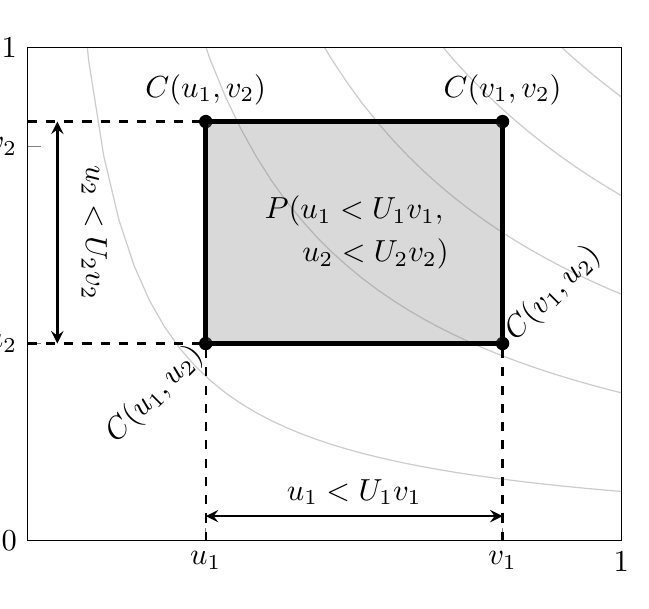
\begin{tikzpicture}[trim axis left, trim axis right, scale=1.1]
        \begin{axis}[%
            xmin=0, xmax=1,
            ymin=0, ymax=1,
            xtick={0.3, 0.8, 1},
            xticklabels={$u_1$, $v_1$, $1$},
            ytick={0, 0.4, 0.8, 1},
            yticklabels={$0$, $u_2$, $v_2$, $1$},
            xtick pos=left,
            ytick pos=left],
            
            \addplot[domain=0:1,samples=40,opacity=0.2]({x},{0.1/x});
            \addplot[domain=0:1,samples=40,opacity=0.2]({x},{0.3/x});
            \addplot[domain=0:1,samples=40,opacity=0.2]({x},{0.5/x});
            \addplot[domain=0:1,samples=40,opacity=0.2]({x},{0.7/x});
            \addplot[domain=0:1,samples=40,opacity=0.2]({x},{0.9/x});
            
            \node (a) at (0.8, 0.85) {};
            \filldraw[black] (a.center) circle (2pt) node[anchor=south,yshift=2pt]{$C(v_1,v_2)$};
            
            \node (b) at (0.3, 0.85) {};
            \filldraw[black] (b.center) circle (2pt) node[anchor=south,yshift=2pt]{$C(u_1,v_2)$};
            
            \node (c) at (0.3, 0.4) {};
            \filldraw[black] (c.center) circle (2pt) node[anchor=east,rotate=45]{$C(u_1,u_2)$};
            
            \node (d) at (0.8, 0.4) {};
            \filldraw[black] (d.center) circle (2pt) node[anchor=west, rotate=45]{$C(v_1,u_2)$};
            
            \draw[ultra thick, black, fill=gray, opacity=0.3] (c.center) rectangle (a.center);
            \draw[ultra thick, black] (c.center) rectangle (a.center) node[pos=0.5,yshift=7pt]{$P(u_1<U_1\leqslant v_1,$} node[pos=0.5, yshift=-7pt, xshift=7pt]{$u_2<U_2\leqslant v_2)$};
            
            \node (e) at (0, 0.85) {};
            \node (f) at (0, 0.4) {};
            \node (g) at (0.8, 0) {};
            \node (h) at (0.3, 0) {};
            \draw[thick, dashed, black] (e.center) -- (b.center);
            \draw[thick, dashed, black] (f.center) -- (c.center);
            \draw[thick, dashed, black] (g.center) -- (d.center);
            \draw[thick, dashed, black] (h.center) -- (c.center);
            
            \node (m) at (0.3, 0.05) {};
            \node (n) at (0.8, 0.05) {};
            \node (o) at (0.05, 0.85) {};
            \node (p) at (0.05, 0.4) {};
            
            \draw [stealth-stealth, thick, black] (m.center) -- (n.center) node[pos=0.5, above]{$u_1<U_1\leqslant v_1$};
            \draw [stealth-stealth, thick, black] (o.center) -- (p.center) node[pos=0.5, anchor=north, rotate=-90, yshift=20pt]{$u_2<U_2\leqslant v_2$};
        \end{axis}
    \end{tikzpicture}\captionof{figure}{Schematic representation of the H-volume}\par}
    
    \Cref{eq:hvol_link_with_proba} means that the H-volume represent the probability of the event
    \begin{equation*}
        u_1 < U_1\leqslant v_1, ~u_2 < U_2\leqslant v_2
    \end{equation*}
    or in other words, the probability that $(U_1, U_2)$ is in the hyper rectangle $[u_1,v_1]\times[u_2,v_2]$ (the intervals can be open or closed in the continuous case, the probability remains the same). Verifying this result for the $n$-dimensional case can be done similarly. \Cref{ex:hvolume} illustrates how the H-volume can be used to compute the discrete joint mass distribution function in the two-dimensional case. 
\end{remark}

A central theorem regarding copulas is \hyperref[theorem:sklar]{Sklar's Theorem} \cite{sklar_fonctions_1959}:
\begin{theorem}[Sklar's Theorem]\label{theorem:sklar}
    Let $F:\X_1\tdt\X_n\rightarrow[0,1]$ be a multivariate cumulative distribution function, where $\X_i\subseteq\overline{\mathbb{R}}$. The marginals $F_i$ of $F$ are defined as $\forall i\in\opi 1,n\cli , \forall x\in\X_i, F_i(x) = F( +\infty\enum  +\infty, x,  +\infty\enum +\infty)$ where $x$ is the $i$-th component of $F$. If all $F_i$ are continuous, then a unique copula $C$ exists:
    \begin{align}
        \forall (x_1\enum x_n)\in \overline{\mathbb{R}}^n, F(x_1\enum x_n)=C(F_1(x_1)\enum F_n(x_n))\label{eq:sklar_equality}
    \end{align}
    If some $F_i$ are not continuous, then $C$ is unique on the product of the ranges of all $F_i$.
    
    The reverse is also true: any copula applied to univariate cumulative distribution functions yields a multivariate cumulative distribution function whose marginals are the univariate \acrshort{cdf}s.
\end{theorem}

\hyperref[theorem:sklar]{Sklar's Theorem} thus allow to express any multivariate \acrshort{cdf} by means of its marginal \acrshort{cdf}s. Conversely, we can join multiple \acrshort{cdf}s with a copula to create a multivariate \acrshort{cdf}. A copula thus expresses the dependency between a multivariate \acrshort{cdf} and its marginals.
 
\begin{remark}
    For marginals $F_i$ that are not continuous, then there can exist multiple copula $C$ verifying \Cref{eq:sklar_equality}. However, if we note $F_i(\X_i)$ the image of $X_i$ through $F_i$, then there exists a unique copula $C$ on the ranges of images $F_1(\X_1)\tdt F_n(\X_n)$. The restriction of a copula to a subset of $I^n$ containing $0$ and $1$ is called a sub-copula. Because we work in discrete spaces, we will mostly work with sub-copulas, but the difference will be mostly transparent.
\end{remark}

Copulas are very useful to represent the dependencies between multiple uncertain variables. As such, they can play a key role in uncertainty propagation problems, explored in \Cref{chap:propagating}.

\begin{example}[Usefulness of the H-Volume]\label{ex:hvolume}
    This example will illustrate how the H-volume of a copula is used to compute the probability mass function of a multivariate probability. Let us imagine a game where a dealer throws two coins, and we are interested in the joint result of the throws. We consider the two random variables $X_1$ and $X_2$ indicating the results of each throw:
    \begin{align*}
        &X_1=0\text{ if the first coin is heads, otherwise }X_1=1\\
        &X_2=0\text{ if the second coin is heads, otherwise }X_2=1
    \end{align*}
    Let $P_1$ and $P_2$ be the probability distributions of $X_1$ and $X_2$ respectively, and assume that both heads and tails are possible outcomes for both coins. We now consider the joint probability distribution $P$ associated with the random variable $(X_1,~X_2)$, and we want to compute the probability mass distribution of $P$. We denote $F_1$, $F_2$ and $F$ the respective \acrshort{cdf}s of $P_1$, $P_2$ and $P$. With this definition, $F_1$ and $F_2$ are the marginals of $F$, and Sklar's theorem states that there exists a copula $C$ such that $F=C(F_1,~F_2)$. 
    
    The probability mass distribution of $P$ can be computed by using the H-volume. For instance, let us start by computing $P(1,1)$. By noticing the fact that:
    \begin{equation*}
        \{x\in\X~|~X_1(x)=1\}=\{x\in\X~|~F_1(X_1(x))=F_1(1)\}
    \end{equation*}
    we can write that:
    \begin{align*}
        P(X_1 = 1, X_2=1) =& ~P(F_1(X_1)= 1, F_2(X_2) = 1)\\
        =& ~P(F_1(0) < F_1(X_1)\leqslant F_1(1), ~F_2(0) < F_2(X_2)\leqslant F_2(1))
    \end{align*}
    A common result in statistics states that random variables of the form $U_1=F_1(X_1)$ and $U_2=F_2(X_2)$ are uniform on $[0,1]$. We can thus apply the result from \Cref{eq:hvol_link_with_proba}, which yields
    \begin{align*}
        P(X_1 = 1, X_2=1) =& ~P(F_1(0) < U_1 \leqslant F_1(1), ~F_2(0) < U_2 \leqslant F_2(1))\\
        =& ~H^{F_1(1),~F_2(1)}_{F_1(0),~F_2(0)}
    \end{align*}
    The probability of the atom $(1,1)$ is therefore equal to the H-volume computed between \acrshort{cdf}s $(F_1, F_2)$ at $(1, 1)$ and at $(0,0)$. Following a similar reasoning, we can compute the probability of every atom and express them as H-volumes:
    \begin{align*}
        P(X_1=0, X_2=1) =& ~H_{0, F_2(0)}^{F_1(0), F_2(1)}\\
        P(X_1=1, X_2=0) =& ~H_{F_1(0), 0}^{F_1(1), F_2(0)}\\
        P(X_1=0, X_2=0) =& ~H_{0,0}^{F_1(0), F_2(0)}
    \end{align*}
    It is possible to generalize our observation: the probability of an atom $(x_1,~\ldots,~x_n)$ is the H-volume computed between marginals \acrshort{cdf}s $(F_1,~\ldots,~F_n)$ at $(x_1,~\ldots,~x_n)$ and at the marginal atoms that precedes them. If $x_1$ is the smallest number, then the marginal \acrshort{cdf} $F_1$ before it equals $0$, \etc.
    \Cref{ex:copulas} presents numerical applications of this example with different copulas.
\end{example}

It follows from \eqref{eq:cop_hvolume} that a copula is a component-wise increasing mapping. All copulas are actually dominating and dominated by two bounds (called lower and upper Fréchet–Hoeffding bounds):
\begin{align}
    &\forall u_i \in [0,1]^n,\nonumber\\
    &\max(0, 1-n+\sum_{i=1}^n u_i) \leqslant C(u_1\enum u_n) \leqslant \min(u_1\enum u_n)
\end{align}
The upper bound is a copula, usually called the Minimum copula $C_M$. It is used to model co-monotonic variables, \ie variables for which high values occur at the same time (or similarly, where low values tend to occur simultaneously). Co-monotonicity implies a maximal covariance between variables.

The lower bound is a copula only in the case $n=2$, called the \L ukasiewicz copula $C_L(u_1,u_2)=\max(0,u_1+u_2-1)$. It is used to model counter-monotonic variables, \ie variables with a perfect negative dependence between them. This explains why the lower bound is not a copula in dimensions higher than $2$. Indeed, if $X$ has a perfect negative dependence with $Y$ and $Z$, then $Y$ and $Z$ cannot share a perfect negative dependence. However, for every $u_1\enum u_n$, there always exists a copula $C$ attaining the lower bound (which can differ for different $u_1\enum u_n$):
\begin{eqnarray*}
    \forall (u_1\enum u_n)\in[0,1]^n,~\exists C \text{ \st }~C(u_1\enum u_n) = \max(0, 1-n+\sum_{i=1}^n u_i)
\end{eqnarray*}
Independence between variables is modeled by the product copula $C_\Pi$:
\begin{equation*}
    C_\Pi(u_1\enum u_n)=\prod_{i=1}^n u_i = u_1\cdot\ldots\cdot u_n
\end{equation*}
where ``$\cdot$'' refers to the product between two scalars, as the symbol $\times$ is already used for the Cartesian product. The product copula will be used later in \Cref{subsection:product_copula}. Graphical representations of the \L ukasiewicz, product and Min copulas are displayed in \Cref{fig:copulas}. \Cref{ex:copulas} presents a setting where the Product, Minimum and \L ukasiewicz copulas are used to model dependency between random variables.

\begin{example}[Different copulas for different dependencies]\label{ex:copulas}
    Let us try to illustrate how different copulas can represent different dependencies. 
    Consider the same setting as \Cref{ex:hvolume} with two coins being thrown. For the purpose of the example, assume that the dealer throws the coins in a separate room, and comes back to tell the result. We thus never see if he is cheating or not. He only provides us this piece of information: coins seems fair when looked at separately. We therefore have the following marginals:
    \begin{eqnarray*}
    \begin{cases}
        P_1(\text{heads}) = P_1(0) = 0.5\\
        P_1(\text{tails}) = P_1(1) = 0.5\\
    \end{cases}
    \qquad\text{ and }\qquad
    \begin{cases}
        P_2(\text{heads}) = P_2(0) = 0.5\\
        P_2(\text{tails}) = P_2(1) = 0.5
    \end{cases}
    \end{eqnarray*}
    
    \begin{itemize}
        \item Assume that the dealer is not cheating and that the two coin throws are independent. In that case, the product copula $C_\Pi(u,v)=u\cdot v$ must be used to represent the independence between variables.
        Using results from the previous example, it holds that:
        \begin{align*}
            P(1,1) =& H_{F_1(1), F_2(1)}^{F_1(0), F_2(0)} = 1\cdot1 - 0.5\cdot1 - 1\cdot0.5 + 0.5\cdot0.5\\
            =& 0.25\\
            P(1,0) =& H_{F_1(0), 0}^{F_1(1), F_2(0)} = 0.25 \\
            P(0,1) =& H_{0, F_2(0)}^{F_1(0), F_2(1)} = 0.25 \\
            P(0,0) =& H_{0, 0}^{F_1(0), F_2(0)} = 0.25
        \end{align*}
        Remark that we indeed find the same results as if we directly multiplied the marginal probability mass distributions: $P(1,1) = P_1(1)\cdot P_2(1)$, \etc. We thus observe the famous result: if $P_1$ and $P_2$ are independent, then $P=P_1\cdot P_2$.
        
        \item Imagine now that the dealer is not being fair, and actually forces the second throw to land on the same side as the first one (the coins will still seem fair when looked at separately). This kind of dependency is modeled by the Minimum copula $C_M(u,v)=\min(u,v)$. In this case, the joint probability is computed as follows: 
		\begin{align*}
            P(1,1) =& H_{F_1(1), F_2(1)}^{F_1(0), F_2(0)} = \min(1,1) - \min(0.5,1) - \min(1,0.5) + \min(0.5,0.5)\\
            =& 0.5\\
            P(1,0) =& H_{F_1(0), 0}^{F_1(1), F_2(0)} =\min(1,0.5) - \min(1, 0) - \min(0.5,0.5) + \min(0,0.5)\\
            =& 0\\
            P(0,1) =& H_{0, F_2(0)}^{F_1(0), F_2(1)} = 0 \\
            P(0,0) =& H_{0, 0}^{F_1(0), F_2(0)} = \min(0.5,0.5)=0.5
        \end{align*}
        The values taken by the joint probability are now completely different from the independence case. We see that values $(0,1)$ and $(1,0)$ are indeed impossible to obtain, while $(1,1)$ and $(0,0)$ are equiprobable.
        
		\item Imagine now that the dealer is still not being fair, but this time forces the second coin to land on the first coin's opposite side. In other words, if the first coin lands on heads, then the dealer puts the second coin on tails, and inversely. Looking at marginal distributions separately will still suggest that the coins are fair. However, they appear fully counter-monotone when looked at jointly. In this case, the dependency is modeled by the \L ukasiewicz copula $C_L(u,v)=\max(0,u+v-1)$, and the joint probability equals:
		\begin{align*}
            P(1,1) =& H_{F_1(1), F_2(1)}^{F_1(0), F_2(0)} = \max(0, 1+1-1) - \max(0, 0.5+1-1)\\
            &- \max(0, 1+0.5-1) + \max(0, 0.5+0.5-1)\\
            =& 0\\
            P(1,0) =& H_{F_1(0), 0}^{F_1(1), F_2(0)} =\max(0, 1+0.5-1) - \max(0, 1+0-1)\\
            &- \max(0, 0.5+0.5-1) + \max(0, 0+0.5-1)\\
            =& 0.5\\
            P(0,1) =& H_{0, F_2(0)}^{F_1(0), F_2(1)} = 0.5 \\
            P(0,0) =& H_{0, 0}^{F_1(0), F_2(0)} = \max(0, 0.5+0.5-1)=0
        \end{align*}
        The values taken by the joint probability is now completely different than in the other cases. We see that values $(1,1)$ and $(0,0)$ are indeed impossible to obtain, while $(0,1)$ and $(1,0)$ are equiprobable.
	\end{itemize}
	Those three cases indicate how copulas can represent very different dependency structures from the same marginals. It also makes it intuitive that the \L ukasiewicz copula only allows values that are ``opposite'', whereas the Minimum copula only allows values that are similar. In those examples, the dependency is so important that knowing the result of one coin throw determines the result of the second, which is therefore modeled by extreme copulas, \ie the upper and lower Fréchet-Hoeffding bounds.  We will see in the following that there are other families of copula that allow less ``extreme'' dependencies.
\end{example}

To complete this overview of copulas, let us present other copulas that can be generated using a single parameter $\theta$ in the case $n=2$. Some famous families of copulas are presented in \Cref{tab:family_of_copula}. Those families are quite common in the literature, but this list is not exhaustive.

Another important family of copulas is the family of Gaussian copulas. Each Gaussian copula is generated with a correlation matrix $R\in[-1,1]^{(n,n)}$:
\begin{align}
    C_R(u_1\enum u_n)=\Phi_R(\Phi^{-1}(u_1)\enum \Phi^{-1}(u_n))
\end{align} where $\Phi_R$ is the joint multivariate cumulative distribution function of a Gaussian variable with correlation matrix $R$, and $\Phi^{-1}$ is the inverse cumulative distribution function of a univariate Gaussian variable. We do not know an exact form for $\Phi_R$, but we can compute it by integrating its associated Gaussian \acrshort{pdf}:
\begin{align}
   \Phi_R&(\Phi^{-1}(u_1)\enum \Phi^{-1}(u_n)) =\nonumber\\ &\int_{-\infty}^{\Phi^{-1}(u_1)}\ldots\int_{-\infty}^{\Phi^{-1}(u_n)}\frac{1}{\sqrt{(2\pi)^{n}|R|}}\exp\left(-\frac{1}{2}\begin{bmatrix}x_1 & \ldots & x_{n}\end{bmatrix}R^{-1}\begin{bmatrix}x_1 \\ \ldots \\ x_{n}\end{bmatrix}\right)dx_1\ldots dx_n
\end{align}
Where $|R|$ is the determinant of $R$. This family of copulas will be used in \Cref{sec:sources_of_uncertainty} to model the dependency between the random intensities of pixels of stereo images, for instance. 
\begin{remark}
    The product copula is actually a Gaussian copula with the identity matrix $\mathbb{I}_n$ as its covariance matrix:
    \begin{align*}
        \Phi_R&(\Phi^{-1}(u_1)\enum \Phi^{-1}(u_n)) =\\ &\int_{-\infty}^{\Phi^{-1}(u_1)}\ldots\int_{-\infty}^{\Phi^{-1}(u_n)}\frac{1}{\sqrt{(2\pi)^{n}|\mathbb{I}_n|}}\exp\left(-\frac{1}{2}\begin{bmatrix}x_1 & \ldots & x_{n}\end{bmatrix}\mathbb{I}_n^{-1}\begin{bmatrix}x_1 \\ \ldots \\ x_{n}\end{bmatrix}\right)dx_1\ldots dx_n\\
        =& \int_{-\infty}^{\Phi^{-1}(u_1)}\ldots\int_{-\infty}^{\Phi^{-1}(u_n)}\frac{1}{\sqrt{(2\pi)^{n}}}\exp(-\frac{1}{2}\sum_{i=1}^nx_i^2)dx_1\ldots dx_n\\
        =& \int_{-\infty}^{\Phi^{-1}(u_1)}\frac{1}{\sqrt{(2\pi)}}\exp(-\frac{1}{2}x_1^2)dx_1\ldots\int_{-\infty}^{\Phi^{-1}(u_n)}\frac{1}{\sqrt{(2\pi)}}\exp(-\frac{1}{2}x_n^2)dx_n\\
        =& \int_{-\infty}^{\Phi^{-1}(u_1)}\Phi'(x_1)dx_1\ldots\int_{-\infty}^{\Phi^{-1}(u_n)}\Phi'(x_n)dx_n\\
        =& ~u_1\ldots u_n
    \end{align*}
\end{remark}

\begin{figure}
    \centering
        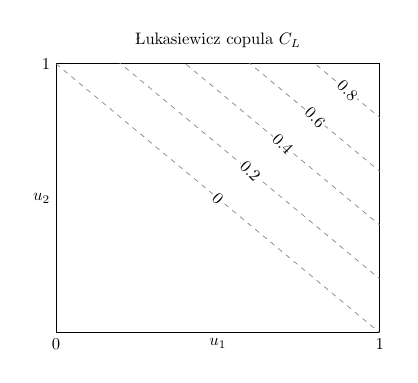
\begin{tikzpicture}[scale=0.6]
        \begin{axis}[
            xmin=0,xmax=1,
            ymin=0,ymax=1,
            xtick={0, 0.5, 1},
		    xticklabels={$0$, $u_1$, $1$},
		    ytick={0.5, 1},
		    yticklabels={$u_2$, $1$},
		    xtick style={draw=none},
		    ytick style={draw=none},
            title={\L ukasiewicz copula $C_L$},
            ]
            \addplot [domain=0:1,samples=40,style=dashed,color=gray]({x},{1-x});
            \addplot [domain=0:1,samples=40,style=dashed,color=gray]({x},{1.2-x}); 
            \addplot [domain=0:1,samples=40,style=dashed,color=gray]({x},{1.4-x}); 
            \addplot [domain=0:1,samples=40,style=dashed,color=gray]({x},{1.6-x}); 
            \addplot [domain=0:1,samples=40,style=dashed,color=gray]({x},{1.8-x});

            \node[rotate=-45, fill=white, rounded corners=2pt, inner sep=1pt] (x) at (0.5, 0.5) {0};
            \node[rotate=-45, fill=white, rounded corners=2pt, inner sep=1pt] (x) at (0.6, 0.6) {0.2};
            \node[rotate=-45, fill=white, rounded corners=2pt, inner sep=1pt] (x) at (0.7, 0.7) {0.4};
            \node[rotate=-45, fill=white, rounded corners=2pt, inner sep=1pt] (x) at (0.8, 0.8) {0.6};
            \node[rotate=-45, fill=white, rounded corners=2pt, inner sep=1pt] (x) at (0.9, 0.9) {0.8};
        \end{axis}
        \end{tikzpicture}\quad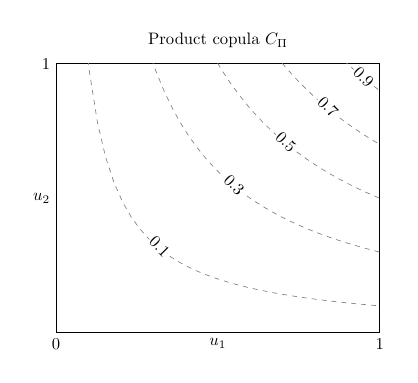
\begin{tikzpicture}[scale=0.6]
        \begin{axis}[
            xmin=0,xmax=1,
            ymin=0,ymax=1,
            xtick={0, 0.5, 1},
		    xticklabels={$0$, $u_1$, $1$},
		    ytick={0.5, 1},
		    yticklabels={$u_2$, $1$},
		    xtick style={draw=none},
		    ytick style={draw=none},
            title={Product copula $C_\Pi$},
            ]
            \addplot[domain=0:1,samples=40,style=dashed,color=gray]({x},{0.1/x});
            \addplot[domain=0:1,samples=40,style=dashed,color=gray]({x},{0.3/x}); 
            \addplot[domain=0:1,samples=40,style=dashed,color=gray]({x},{0.5/x}); 
            \addplot[domain=0:1,samples=40,style=dashed,color=gray]({x},{0.7/x}); 
            \addplot[domain=0:1,samples=40,style=dashed,color=gray]({x},{0.9/x});

            \node[rotate=-45, fill=white, rounded corners=2pt, inner sep=1pt] (x) at (0.32, 0.32) {0.1};
            \node[rotate=-45, fill=white, rounded corners=2pt, inner sep=1pt] (x) at (0.55, 0.55) {0.3};
            \node[rotate=-45, fill=white, rounded corners=2pt, inner sep=1pt] (x) at (0.71, 0.71) {0.5};
            \node[rotate=-45, fill=white, rounded corners=2pt, inner sep=1pt] (x) at (0.84, 0.84) {0.7};
            \node[rotate=-45, fill=white, rounded corners=2pt, inner sep=1pt] (x) at (0.95, 0.95) {0.9};
            
        \end{axis}
        \end{tikzpicture}\quad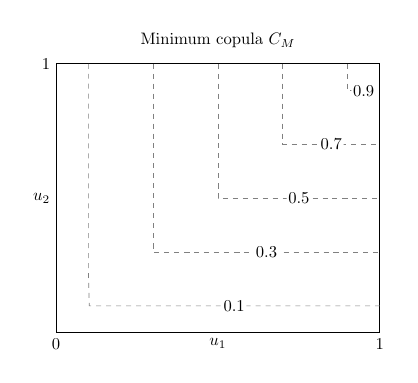
\begin{tikzpicture}[scale=0.6]
        \begin{axis}[
            xmin=0,xmax=1,
            ymin=0,ymax=1,
            xtick={0, 0.5, 1},
		    xticklabels={$0$, $u_1$, $1$},
		    ytick={0.5, 1},
		    yticklabels={$u_2$, $1$},
		    xtick style={draw=none},
		    ytick style={draw=none},
            title={Minimum copula $C_M$},
            ]
            \addplot [domain=0:1,samples=40,style=dashed,color=gray]({max(x, 0.1)},{max(1-x/0.1,0.1)});
            \addplot [domain=0:1,samples=40,style=dashed,color=gray]({max(x, 0.3)},{max(1-x/0.3,0.3)});
            \addplot [domain=0:1,samples=40,style=dashed,color=gray]({max(x, 0.5)},{max(1-x/0.5,0.5)});
            \addplot [domain=0:1,samples=40,style=dashed,color=gray]({max(x, 0.7)},{max(1-x/0.7,0.7)});
            \addplot [domain=0:1,samples=40,style=dashed,color=gray]({max(x, 0.9)},{max(1-x/0.9,0.9)});

            \node[fill=white, rounded corners=2pt, inner sep=1pt] (x) at (0.55, 0.1) {0.1};
            \node[fill=white, rounded corners=2pt, inner sep=1pt] (x) at (0.65, 0.3) {0.3};
            \node[fill=white, rounded corners=2pt, inner sep=1pt] (x) at (0.75, 0.5) {0.5};
            \node[fill=white, rounded corners=2pt, inner sep=1pt] (x) at (0.85, 0.7) {0.7};
            \node[fill=white, rounded corners=2pt, inner sep=1pt] (x) at (0.95, 0.9) {0.9};
        \end{axis}
        \end{tikzpicture}
    \caption{Bird view of the \L ukasiewicz, product and Min copulas for $n=2$. Dashed gray lines represent isolines of the copulas.}
    \label{fig:copulas}
\end{figure}


{\renewcommand{\arraystretch}{2}%
\begin{table}[!ht]
    \centering
    \begin{tabular}{|c|c|c|c|c|}
        \hline
        Family & $C(u_1,u_2)$ & $\theta \in $ & D-convex & D-concave \\
        \hline\hline
        Ali-Mikhail-Haq & $\frac{u_1u_2}{1-\theta(1-u_1)(1-u_2)}$ & $[-1,1)$ & $\theta\leqslant0$ & $\theta\geqslant 0$ \\
        \hline
        Clayton & $\left[\max(u_1^{-\theta}+u_2^{-\theta}-1,0)\right]^{-1/\theta}$ & $[-1,\infty)\backslash\{0\}$ & $\theta<0$ & $\theta>0$ \\
        \hline
        Frank & $-\frac{1}{\theta}\ln(1+\frac{(e^{-\theta u_1}-1)(e^{-\theta u_2}-1)}{e^{-\theta}-1})$ & $\mathbb{R}\backslash \{0\}$ & $\theta<0$ & $\theta>0$ \\
        \hline
        Gumbel & $u_1u_2\exp(-\theta \ln{u_1}\ln{u_2})$ & $(0,1]$ & $\theta\in(0,1]$  & Never \\
        \hline
    \end{tabular}
    \caption{Examples of families of copulas in the case $n=2$ which can be generated using a parameter \( \theta \). D-convexity/concavity is detailed in the Annex \Cref{sec:dconvexity}}
    \label{tab:family_of_copula}
\end{table}}

\begin{remark}
	As a copula is also a multivariate \acrshort{cdf}, one can imagine an ``imprecise'' copula \cite{montes_sklars_2015} similarly to what can be done with univariate probability distribution (see \Cref{sec:imprecise_probabilities}). Imprecise copulas allow modeling partially known dependencies, but can be hard to manipulate at times, as for instance the lower and upper bounds of an imprecise copula are not necessarily copulas themselves. In this thesis, we will not consider imprecise copulas.
\end{remark}

\subsection{Sampling from a Copula}\label{sec:sampling_copula}
As a copula represents the \acrshort{cdf} of a multivariate random variable, it is possible to sample from it. This section details a method for sampling from copulas in general, and a special method for sampling from Gaussian copulas. \Cref{chap:propagating} will use those methods for Monte Carlo sampling. For simplicity, let us first present a method for sampling in the case $n=2$. Given a copula $C$, and two \acrshort{cdf}s $F_X$ and $F_Y$, a method to generate a pair of observations $(x, y)$ from a joint \acrshort{cdf} $C(F_X, F_Y)$ is the following:

\begin{itemize}
    \item Sample two independent samples $u_1, u_2$ from a uniform distribution on [0,1]
    \item Set $v=\partial C^{-1}(u_2)$ where $\partial C^{-1}$ is the quasi-inverse of the partial derivative of $C$ with respect to its first variable (which exists almost everywhere and is invertible).
    \item We now have a sample $(u_1, v)$ from a multivariate random variable. Its marginals follow a uniform distribution on $[0,1]$, and its associated copula is $C$.
    \item The desired pair is $(x,y) = (F^{-1}_X(u_1), F^{-1}_Y(v))$, with $F_X^{-1}$, $F_Y^{-1}$ being the quasi-inverses of the marginals \acrshort{cdf}s.
\end{itemize}

We do not present the $n$-dimensional general case here as it is a bit more complex, but it can be found in \cite{cherubini_copula_2004}. However, drawing samples from a Gaussian $n$-copula with a correlation matrix $R$ are simpler to obtain:
\begin{itemize}
    \item Compute the Cholesky decomposition $A$ of the correlation matrix $R$
    \item Draw $n$ independent random samples $u=(u_1\enum u_n)'$ from $\mathcal{N}(0,1)$, where $\mathcal{N}$ is the normal distribution.
    \item Set $v=Au$
    \item Set $w_k=\Phi(v_k)$ where $\Phi$ is the univariate normal cumulative distribution function
    \item The desired draw is $(x_1\enum x_n)=(F^{-1}_1(w_1)\enum F^{-1}_n(w_n))$ with $F_i^{-1}$, being the quasi-inverse of the $i$-th marginal \acrshort{cdf}.
\end{itemize}

\begin{conclusion}
    In this chapter, we presented different uncertainty models, whose usage depends on the type of uncertainty and evidence available.  Choosing between the different models is often a trade-off between expressivity, compatibility and ``realism'' of the hypotheses of the considered problem. We also presented a way to combine probabilities by taking into account the dependency between random variables, using copulas. Copulas are well suited for probabilities, but their usage with \acrshort{ip} is more complex. \Cref{chap:joining_credal_sets} will investigate how \acrshort{ip} models can be combined using a copula, and \Cref{chap:propagating} will use copulas and imprecise models in a stereo matching problem.
\end{conclusion}

\clearpage